\section{Case studies}\label{case-studies}\label{sec:cases}

We present four cases that we built as maintainers (Table 5.1). They are worked examples of the framework rather
than a fixed benchmark: each is a starting point for questions about the decision it models, and Section 7.2 lists
the questions we consider open. The cases show how the counterpart changes measured value and how a shortfall divides
into typed action classes, and Section 5.3 runs an external benchmark on the same runtime. We describe Housing,
Procurement and Data center here and specify them in Appendices A--D; Refund appears only in the cross-case comparison.
Each case is a family rather than a fixed task set. It consists of a generator of worlds; a case-specific reference,
which is either a policy that uses only what the deciding side may know or an explicitly labelled full-information
upper bound; an inclusion criterion that keeps the worlds in which the decision matters (its form varies by case;
Appendix E.2); and a set of verifiers. The references differ in what a shortfall means. Against a reachable policy,
the shortfall is the value that a feasible strategy would have kept. Against the best policy given the decider's
information, it is the whole cost of the decisions. Against a full-information bound, it also includes the value of
information that no seat had (Appendix C).

We choose cases by the economic value of the decision rather than by occupation \citep{li2026activities}. An activity qualifies when its
value is decided rather than produced, when a counterparty has its own interest and private information, and when the
result can be scored within a world against a computed reference. The four examples lie in two of the five
transaction classes introduced in §3, business and household purchases. We chose them to span the kinds of verifier
and counterpart, not to sample a representative distribution.

\renewcommand{\thetable}{5.1}
\begin{longtable}[]{@{}
  >{\raggedright\arraybackslash}p{(\linewidth - 8\tabcolsep) * \real{0.2000}}
  >{\raggedright\arraybackslash}p{(\linewidth - 8\tabcolsep) * \real{0.2000}}
  >{\raggedright\arraybackslash}p{(\linewidth - 8\tabcolsep) * \real{0.2000}}
  >{\raggedright\arraybackslash}p{(\linewidth - 8\tabcolsep) * \real{0.2000}}
  >{\raggedright\arraybackslash}p{(\linewidth - 8\tabcolsep) * \real{0.2000}}@{}}
\caption{\textbf{The four cases. Each case is scored in its own units against the reference given in the last column.}}\label{tab:5.1}\tabularnewline
\toprule\noalign{}
\begin{minipage}[b]{\linewidth}\raggedright
Case
\end{minipage} & \begin{minipage}[b]{\linewidth}\raggedright
Real setting
\end{minipage} & \begin{minipage}[b]{\linewidth}\raggedright
What the agent decides
\end{minipage} & \begin{minipage}[b]{\linewidth}\raggedright
Who it faces
\end{minipage} & \begin{minipage}[b]{\linewidth}\raggedright
Scored against
\end{minipage} \\
\midrule\noalign{}
\endhead
\bottomrule\noalign{}
\endlastfoot
Housing & informal rental listings & which listing to inspect, what to offer, and whether to sign when some listings are lemons & scripted landlords; other tenants take listings it leaves & a scripted tenant that uses only what the tenant knows \\
Procurement & wholesale sourcing & pay more for an established supplier, or test a cheaper newcomer, before a deadline & scripted suppliers & the best plan given what the buyer knows, solved exactly \\
Data center & AI-infrastructure contracting & which risk clauses to change, what price to name, and when to sign or walk away & the other side: a script, another model or the same model & the best agreement at both sides' true costs, which neither side knows \\
Refund & customer refund claims & what to ask, decide and pay on a claim under a written policy & the other parties to the claim, scripted & a hand-written correct resolution \\
\end{longtable}

We report how much room each case leaves as a share of that case's own reference value. Tables 5.2 to 5.4 give each
subject's result and gap in this form, and Figure 5.2 divides the gap by action class in the case's own units. The
cases use four of the kinds of check defined with the runner's measurement layer (§4): an answer key, stated rules,
the value of the best policy or a bound, and relative standing against another agent. None uses a rubric. Every score
is computed by code, with no model in the loop. The kernel's replay recomputes each receipt's own score from its
sealed events, whereas the headline measures of Housing and Procurement are computed by case code outside that
certificate (Appendix F.2). Table E.1 lists every check.

\subsection{Results}\label{results}

Each result below is bounded by its case's quality-control gates; Table 6.1 gives every comparison's status, and
Section 6 describes the gates. ``Pre-registered'' below describes how a comparison was run, namely with its analysis
committed to the repository before any episode; it does not describe the case. The results compare the named
subjects on these worlds and are not qualified benchmark scores.

\textbf{Housing.} The structure follows informal rental markets on social platforms such as RedNote. Listings are posted
with photos that a tenant cannot check before viewing, a viewing costs time, and good listings are often taken while
the tenant decides. We set the rents, the lemon share and the inspection cost ourselves; they are not drawn from
platform data. A tenant chooses among four listings, two of which are lemons. It knows its own value v\_ℓ for each
listing if sound, but not which two are lemons; each of the six pairs is equally likely. In each of three rounds it
may pay \$25 to inspect one listing, make one offer, and sign or walk away from a lease it is offered, while each
listing it did not bid on is taken by outside demand with probability ½. Signing listing ℓ at rent x after k
inspections pays

\[ \text{v\_ℓ − 1,000·𝟙[ℓ is a lemon] − x − 25k,} \tag{1} \]

and signing nothing pays −25k. The difficulty lies in information. A listing worth \$400 more than its ask if sound is
worth 400 − ½·1,000 = −\$100 if signed blind at the ask, but ½·400 − 25 = +\$175 if it is inspected first and signed only
when sound; inspecting a second listing takes another round, in which each listing not bid on may be taken. A
landlord's reply can reveal a lemon at no cost: every world is played against one landlord kind whose reply to a low
offer reveals a lemon and one whose reply does not. We score a blind signing at its expected value given what the
tenant knew, so that the score follows the decision rather than the draw, with the odds conditioned on every
informative landlord reply. This corrected measure is introduced in this paper; v14's pre-registered measure
conditioned on only one landlord kind (Appendix E.4). The comparison reported here, v15, was pre-registered before any
of its artifacts and changes four things from v14. Each included world is screened so that the best informed tenant
beats a simple inspect-then-sign rule by at least \$25 (119 of 437 candidate main worlds failed); the tenant's task
prompt states how landlords price; the corrected measure is primary from the start; and each receipt scores the
deciding tenant. Its holdout of 40 worlds changes one mechanism, outside demand at 0.3 a round, and its task prompt
says so.

\renewcommand{\thetable}{5.2}
\begin{longtable}[]{@{}
  >{\raggedright\arraybackslash}p{(\linewidth - 8\tabcolsep) * \real{0.1579}}
  >{\raggedleft\arraybackslash}p{(\linewidth - 8\tabcolsep) * \real{0.2105}}
  >{\raggedleft\arraybackslash}p{(\linewidth - 8\tabcolsep) * \real{0.2105}}
  >{\raggedleft\arraybackslash}p{(\linewidth - 8\tabcolsep) * \real{0.2105}}
  >{\raggedleft\arraybackslash}p{(\linewidth - 8\tabcolsep) * \real{0.2105}}@{}}
\caption{\textbf{Housing v15, main evaluation set of 260 worlds (200 with the favourite a lemon, 60 sound): seat 0's net payoff under the corrected measure as a share of what the best informed tenant earns in the same worlds (\$307 a world on the main evaluation set), averaged over the two landlord arms. Differences are in percentage points of that value, with 95\% intervals over worlds. The comparison was pre-registered before any v15 artifact; dollar values are in the results note, and the comparison with v14 is in Table E.13. Sol 6.1 and Opus 5.5 played the same worlds through their command-line tools in a pre-registered addendum, outside v15's contrasts.}}\label{tab:5.2}\tabularnewline
\toprule\noalign{}
\begin{minipage}[b]{\linewidth}\raggedright
\end{minipage} & \begin{minipage}[b]{\linewidth}\raggedleft
Gemini 3.8 Flash
\end{minipage} & \begin{minipage}[b]{\linewidth}\raggedleft
GPT-6 Luna
\end{minipage} & \begin{minipage}[b]{\linewidth}\raggedleft
Sol 6.1 (Codex), addendum
\end{minipage} & \begin{minipage}[b]{\linewidth}\raggedleft
Opus 5.5 (Claude Code), addendum
\end{minipage} \\
\midrule\noalign{}
\endhead
\bottomrule\noalign{}
\endlastfoot
Share of the best informed tenant's value & 78.7\% & 62.9\% & 90.4\% & 80.4\% \\
Favourite is a lemon / sound & 68.8\% / 100.0\% & 46.8\% / 97.3\% & 85.9\% / 100.0\% & 71.2\% / 100.0\% \\
Minus \texttt{inspect\_\allowbreak{}then\_\allowbreak{}sign} (the pre-registered beatability baseline), points & +29.3 {[}+24.7, +33.8{]} & +13.4 {[}+8.2, +18.6{]} & +40.9 {[}+36.2, +45.6{]} & +30.9 {[}+26.3, +35.5{]} \\
Minus \texttt{inspect\_\allowbreak{}lowball} (v14's reachable reference), points & −16.6 {[}−20.8, −12.5{]} & −32.5 {[}−37.8, −27.3{]} & −5.0 {[}−8.0, −2.0{]} & −15.0 {[}−18.9, −11.0{]} \\
Holdout (40 worlds, outside demand at 0.3) & 79.3\% & 61.1\% & 88.0\% & 80.1\% \\
\end{longtable}

Relative to the best informed tenant's value, the full-information ceiling is 121\%, \texttt{inspect\_\allowbreak{}lowball} earns 95\% and
\texttt{inspect\_\allowbreak{}then\_\allowbreak{}sign} 49\%. Under the analysis pre-registered before any episode, Gemini leads Luna by 15.9 points
{[}11.3, 20.4{]} of that value. The difference is detected but is not shown to exceed the pre-registered \$50 band
(16.3 points). The A/A arm, in which Luna runs twice under two names with different seeds, differs by −1.6 points
{[}−6.1, +2.9{]}, inside the band, which indicates that the band is calibrated. Both models beat the pre-registered
baseline, and both remain below v14's reachable rule and the best informed tenant. Almost the whole shortfall arises in
worlds where the favourite listing is a lemon: there Gemini keeps 69\% and Luna 47\% of what the best informed tenant
earns, against 100\% and 97\% where the favourite is sound. In those worlds Luna signs blind twice as often as Gemini
(230 against 114 blind signings in 600 episodes). In the holdout Gemini leads by 18.2 points {[}5.8, 30.6{]}. All 1,720
episodes completed and were verified by replay (\$8.64). Because v15 differs from v14 in four ways at once (the
screened evaluation set, the stated pricing rule, the corrected measure as primary, and seat-0 receipts), its levels
are not comparable with v14's, and we attribute no change between them to the models or to any single difference.
GLM 5.3 Flash was excluded at the pre-run profile check, because its provider now serves a different quantization from
the one v14 pinned. A pre-registered addendum ran it on another provider serving v14's quantization (600 of 600
episodes, verified by replay); we report it beside v15 and outside its pre-registered contrasts. On the main evaluation
set GLM keeps 53.9\% of the best informed tenant's value and does not beat \texttt{inspect\_\allowbreak{}then\_\allowbreak{}sign} at the pre-registered
98.3\% level (+4.5 points {[}−4.4, +13.3{]}); descriptively, it trails Luna by 8.9 points {[}1.6, 16.2{]} and Gemini by 24.8
{[}19.0, 30.5{]}. A second pre-registered addendum ran Sol 6.1 and Opus 5.5 through their command-line tools on the same
600 episodes each (all completed and verified by replay), likewise outside v15's contrasts. Sol keeps 90.4\% of the
best informed tenant's value and comes closest to v14's reachable rule (5.0 points below it); Opus keeps 80.4\%. Both
beat \texttt{inspect\_\allowbreak{}then\_\allowbreak{}sign} at the 98.3\% level. Sol leads Opus by 10.0 points {[}7.4, 12.6{]}, and Opus is statistically
indistinguishable from Gemini (+1.6 {[}−0.3, +3.6{]}). As with the flash models, nearly all of each model's shortfall arises
in worlds whose favourite is a lemon.

\textbf{Procurement.} The structure follows wholesale sourcing on B2B platforms such as Alibaba's 1688. A displayed price
is not a quote, a listing's quality is known only after it is checked, and new sellers of one kind often buy from the
same factory. A buyer owes 50 kits by a deadline and awards the order to one supplier: either a recorded supplier with
a long clean record or one of three newcomers. Each newcomer is good, late or poor. The buyer knows only the odds,
which are read from the record of the newcomer's seller kind, and that newcomers of one kind share a source with a
stated probability (0.5 to 0.95), in which case they are all of the same type. Two features follow our own sourcing on
1688. A newcomer's price relative to the recorded supplier's is drawn from the price gaps in that record, so a
newcomer is dearer about half the time, and a newcomer answers a quote request only a third of the time. We set the
case's other quantities ourselves. Among up to ten actions the buyer may request a quote (\$2 and a day; an answered
quote exposes a late supplier), request a sample (\$20 to \$240 and three days; it always arrives and exposes a poor
supplier), look up a listing's registered factory (\$1; two lookups in one kind show whether the kind shares a
source), award the order, or defer. An award that delivers k kits on time earns

\[ \text{37k − 12(50 − k) − cost of the order − cost of the information bought,} \tag{2} \]

and an award that delivers fewer than 40 kits, as a late or poor supplier does, earns −\$600 less the information
bought (Appendix A.2).

The difficulty is a test worth taking only for what it reveals about another supplier. Every world in the evaluation
set is one in which a rule that plans a single newcomer's test exactly (what to request first, how often to repeat an
unanswered quote, and when to give up) pays the premium, while the best policy tests a newcomer first and beats paying
the premium by at least 10\%. In one world the recorded supplier asks \$24.95. A newcomer asks \$12.47, but its sample
costs \$200 and its odds are 0.20 good, 0.15 late and 0.65 poor, so testing it on its own loses money. A second
newcomer of the same seller kind asks \$26.87, more than the recorded supplier, so it is never worth buying; but its
sample costs \$30, and the two share a source with probability 0.95. Once the cheap newcomer's quote has come back
clean, a sound sample of the dear newcomer raises the cheap newcomer's probability of being good to 0.94, and a poor
sample lowers it to 0.01. The best policy therefore requests a quote from the cheap newcomer; if the quote comes back
clean, it samples the dear newcomer, looks both up, and only then pays for the \$200 sample. It earns 11.8\% more than
paying the premium. Every action is charged the value it gave up relative to the exact best informed policy at that
point.

\renewcommand{\thetable}{5.3}
\begin{longtable}[]{@{}
  >{\raggedright\arraybackslash}p{(\linewidth - 6\tabcolsep) * \real{0.2000}}
  >{\raggedleft\arraybackslash}p{(\linewidth - 6\tabcolsep) * \real{0.2667}}
  >{\raggedleft\arraybackslash}p{(\linewidth - 6\tabcolsep) * \real{0.2667}}
  >{\raggedleft\arraybackslash}p{(\linewidth - 6\tabcolsep) * \real{0.2667}}@{}}
\caption{\textbf{Procurement, the 20 worlds of the pre-registered test, two plays each: the share of the gap between paying the premium and the best policy that each subject closes (a mean over worlds, each world the mean of its plays, with 95\% t intervals), the loss per world relative to the best policy, and the number of plays that touched a newcomer. The worlds were drawn, and the test on Sol pre-registered, before any play. In every world, a rule that plans one newcomer's test exactly pays the premium and closes none of the gap.}}\label{tab:5.3}\tabularnewline
\toprule\noalign{}
\begin{minipage}[b]{\linewidth}\raggedright
\end{minipage} & \begin{minipage}[b]{\linewidth}\raggedleft
Share of the gap closed
\end{minipage} & \begin{minipage}[b]{\linewidth}\raggedleft
Loss per world
\end{minipage} & \begin{minipage}[b]{\linewidth}\raggedleft
Plays touching a newcomer
\end{minipage} \\
\midrule\noalign{}
\endhead
\bottomrule\noalign{}
\endlastfoot
Sol 6.1 (Codex) & 35\% {[}18, 52{]}, p = 0.0003 & \$32.51 & 26 of 40 \\
Opus 5.5 (Claude Code) & 0\% in every world & \$51.25 & 0 of 40 \\
Gemini 3.8 Flash & 0\% in every world & \$51.25 & 0 of 40 \\
GPT-6 Luna & −14\% {[}−21, −7{]} & \$58.10 & 0 of 40 \\
\emph{Exact rules on the same worlds} & & & \\
Paying the premium; a rule that plans one newcomer's test & 0\% & \$51.25 & \\
Shortcut: sample the newcomer with the cheapest sample first, ignoring seller kinds & 33\% & \$33.46 & \\
A rule that may test two newcomers & 82\% & \$8.38 & \\
\end{longtable}

\begin{figure}[htbp]\centering\renewcommand{\thefigure}{5.1}
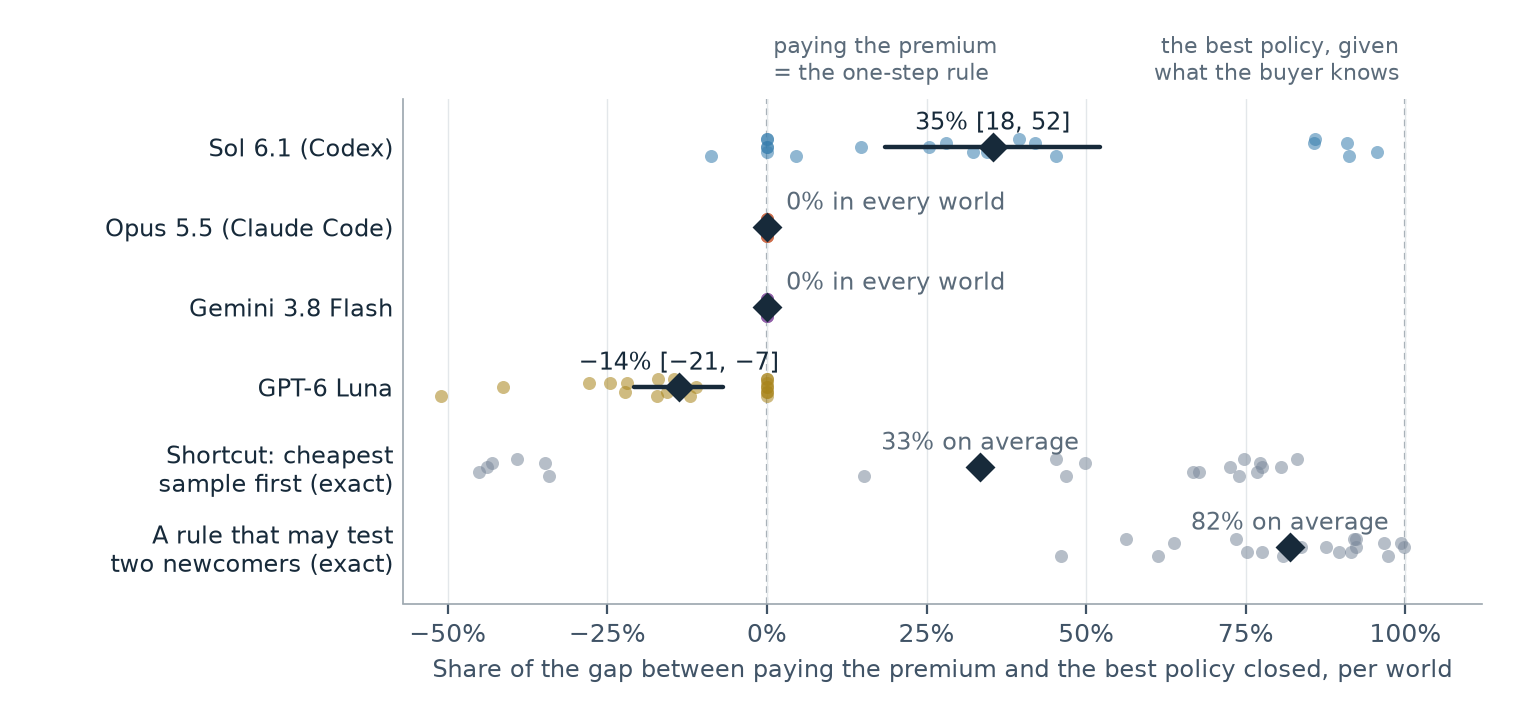
\includegraphics[width=\linewidth]{figures/procurement_v3_gap_closed.png}
\caption{\textbf{Procurement, the 20 pre-registered worlds: the share of the gap between paying the premium and the best policy closed, world by world.} Each dot is
one world, the mean of its two plays; diamonds are means and bars are 95\% t intervals. Paying the premium and a rule
that plans one newcomer's test exactly both sit at 0\% in every world. Opus and Gemini close none of the gap in any
world; Luna's orders of 50 units where 55 was best leave it below paying the premium. The gray rows are exact rules:
the shortcut that ignores seller kinds and first samples the newcomer whose sample is cheapest, and a rule allowed to
test two newcomers.}
\label{fig:5.1}
\end{figure}

Sol 6.1 closed 35\% of the gap (95\% t interval 18--52\%, p = 0.0003), whereas a rule that plans one newcomer's test
exactly closes none. This was the one test we pre-registered before any play, and the claim holds; it concerns Sol
alone. Its play varies by world (Figure 5.1): it closes most of the gap in some worlds and none in others. The other
three models never touched a newcomer. Opus 5.5 and Gemini 3.8 Flash paid the premium in every play; GPT-6 Luna did
too, but it ordered 50 units where 55 was best in 15 of its 40 plays, which leaves it below paying the premium. A
shortcut that ignores seller kinds and first samples the newcomer whose sample is cheapest closes 33\%, about Sol's
share, but Sol does not play that shortcut: it opens with the shortcut's move in 2 of 40 plays, and its tests follow
price. The moves the case is built around are rare in its play: it tests a second newcomer in 7 of 40 plays and looks
up a source in 4. A rule allowed to test two newcomers closes 82\%, so the remaining headroom lies in planning one test
beyond the one in hand.

Further runs on this evaluation set are reported in Appendix E.4 (Table E.15): a development pilot, the
pre-registered worlds at the earlier evaluation set's more favourable odds, and a task prompt corrected for four
wording defects. None of them changes this picture. One of them bears on why Opus never tests. In a check with no
play, Opus was asked how likely a newcomer is to be sound once another newcomer of its kind has passed or failed a
sample, with and without a clean quote of its own first, and it answered all 18 questions within 0.05 of the exact
value, as Sol did. Opus therefore applies the sharing rule correctly when asked, but does not plan with it. These runs
used the case's environment from a development branch, which is now on the main branch with its registration; every
published receipt replays through the runtime's command line (Appendix F.1). On an earlier evaluation set, in which
quotes always arrive and newcomers never share a source, performance saturates: a rule that looks one test ahead comes
within 0.01\% of the best policy (Appendix E.4, Table E.14).

\textbf{Data center.} The structure follows a real AI-infrastructure engagement in which a system integrator bundles
hardware, data-center space, staffing and software into a working system for a client. Hardware can arrive late or
defective, the site may not be ready, and the contract's warranty, delay-damages, liability-cap, site-readiness,
deposit and burn-in clauses decide who bears each cost. We set the costs, probabilities and prices ourselves. Client
and integrator negotiate one agreement, consisting of a position on each of the eight clauses (600 distinct
agreements) and an all-in price p.~Each side knows its own cost of carrying risk and only the probability distribution
of the other's: the integrator's pre-staging cost and risk charge, and the client's risk charge. Over six alternating
moves, a side may redline any clauses and name a price, sign the standing version, or walk away, and each redline
after the first move costs \$25k. In thousands of dollars and net of redline fees, a signed agreement c pays the
integrator and the client, respectively,

\[ \text{π\_I = p − C\_I(c) − 500,  π\_C = O\_C − p − C\_C(c),} \tag{3} \]

where 500 is the integrator's outside option, O\_C the client's, and C\_I and C\_C each side's expected cost of the risks
that the clauses leave with it, marked up by its risk charge; no deal pays only the fees. The difficulty is that price
only divides the value, while the clauses determine how much value there is, and the best clauses depend on what the
other side hides. Burn-in, for example, costs the integrator \$40k and, in one world, costs the client a week's delay
worth \$110k, and it halves the probability of a \$3 million incident that the client carries. It therefore lowers joint
cost by \$41k for a client with the highest risk charge and raises it by \$19k or \$64k for the other two, and the
integrator cannot tell which client it faces. The comparison reported here (v2) was pre-registered before its runs, on
80 included worlds (from 5,436 scanned), 72 of them with a mutually beneficial deal. Both command-line tools were
isolated, the client's task prompt states its walk-away point, and a world is included only if the integrator has at
least \$25k of room over a price-only rule. An earlier pre-registered comparison (v1) did none of these three things;
it is reported in Appendix E.4 (Table E.16), and development results remain in Tables E.3 and E.7.

\renewcommand{\thetable}{5.4}
\begin{longtable}[]{@{}
  >{\raggedright\arraybackslash}p{(\linewidth - 6\tabcolsep) * \real{0.2143}}
  >{\raggedleft\arraybackslash}p{(\linewidth - 6\tabcolsep) * \real{0.2857}}
  >{\raggedright\arraybackslash}p{(\linewidth - 6\tabcolsep) * \real{0.2143}}
  >{\raggedleft\arraybackslash}p{(\linewidth - 6\tabcolsep) * \real{0.2857}}@{}}
\caption{\textbf{Data center, the pre-registered comparison (v2): Sol 6.1 (Codex) and Opus 5.5 (Claude Code). Differences in a seat's earnings above its outside option, at true costs, on the 72 deal worlds, in percentage points of the value available in a deal (the joint surplus of the best agreement, \$309k a world); intervals are 95\%, with Holm correction across the four primary contrasts. Gate 3 passes for the integrator seat; Gates 0, 1, 2, 4 and 5 are partial (Table 6.1).}}\label{tab:5.4}\tabularnewline
\toprule\noalign{}
\begin{minipage}[b]{\linewidth}\raggedright
Primary contrast
\end{minipage} & \begin{minipage}[b]{\linewidth}\raggedleft
Worlds
\end{minipage} & \begin{minipage}[b]{\linewidth}\raggedright
Estimate {[}95\% interval{]}
\end{minipage} & \begin{minipage}[b]{\linewidth}\raggedleft
Holm p
\end{minipage} \\
\midrule\noalign{}
\endhead
\bottomrule\noalign{}
\endlastfoot
Head to head: Sol minus Opus earnings, seat-averaged & 72 deal & +41.7 {[}31.3, 52.0{]} & 6.1e-11 \\
Integrator against the firm client: Sol minus Opus & 72 deal & +7.5 {[}1.7, 13.2{]} & 0.022 \\
Sol as integrator minus the price-only rule & 72 deal & +7.3 {[}2.6, 12.0{]} & 0.008 \\
Opus as integrator minus the price-only rule & 72 deal & −0.2 {[}−5.5, 5.2{]} & 0.95 \\
\end{longtable}

All freeze and run probes were clean, and all 640 negotiations are valid and replayed (\$55.41 at list price). The
head-to-head gap is 41.7 points and the firm-client gap 7.5; each is detected under the Holm correction, and neither is
shown to reach its pre-registered minimum (32.4 and 12.9 points, \$100k and \$40k). Head to head, the opponent changes
with the focal model, whereas the firm-client contrast holds the counterpart policy fixed, which supports a
counterpart-specific reading of the larger gap. As integrator, Sol beats the price-only rule, and Opus earns what the
rule earns. With the walk-away point stated, neither model signs below it as client (0 of 80 for either), and the
client seat separates nothing (+0.8 points {[}−3.2, 4.9{]}).

We computed the best informed turn-by-turn policy after both runs, against the same scripted counterpart
(Appendix C.3). On v2's deal worlds it gives the integrator 63.5\% of the value available at the true client type,
whereas Sol earned 33.8\%, Opus 26.3\% and the price-only rule 26.5\%. Sol therefore captures about 20\% of the room
between the rule and that reference. In both seats and both campaigns, knowing the other side's type is worth less than
1\% of the value available to this policy, so the case measures bargaining against a fixed counterpart far more than
inference about it.

\subsection{Where the shortfall comes from}\label{where-the-shortfall-comes-from}

Figure 5.2 divides each case's shortfall into observed action classes. The components sum to the total under a stated
priority order, and they describe what happened, not its cause. Each panel uses its own reference and units.
Appendix E.5 gives the classification rules and the full subject tables, and Appendix E.7 gives the current Data-center
breakdown and its uncertainty. Table E.10 retains the exact panel values.

\begin{figure}[htbp]\centering\renewcommand{\thefigure}{5.2}
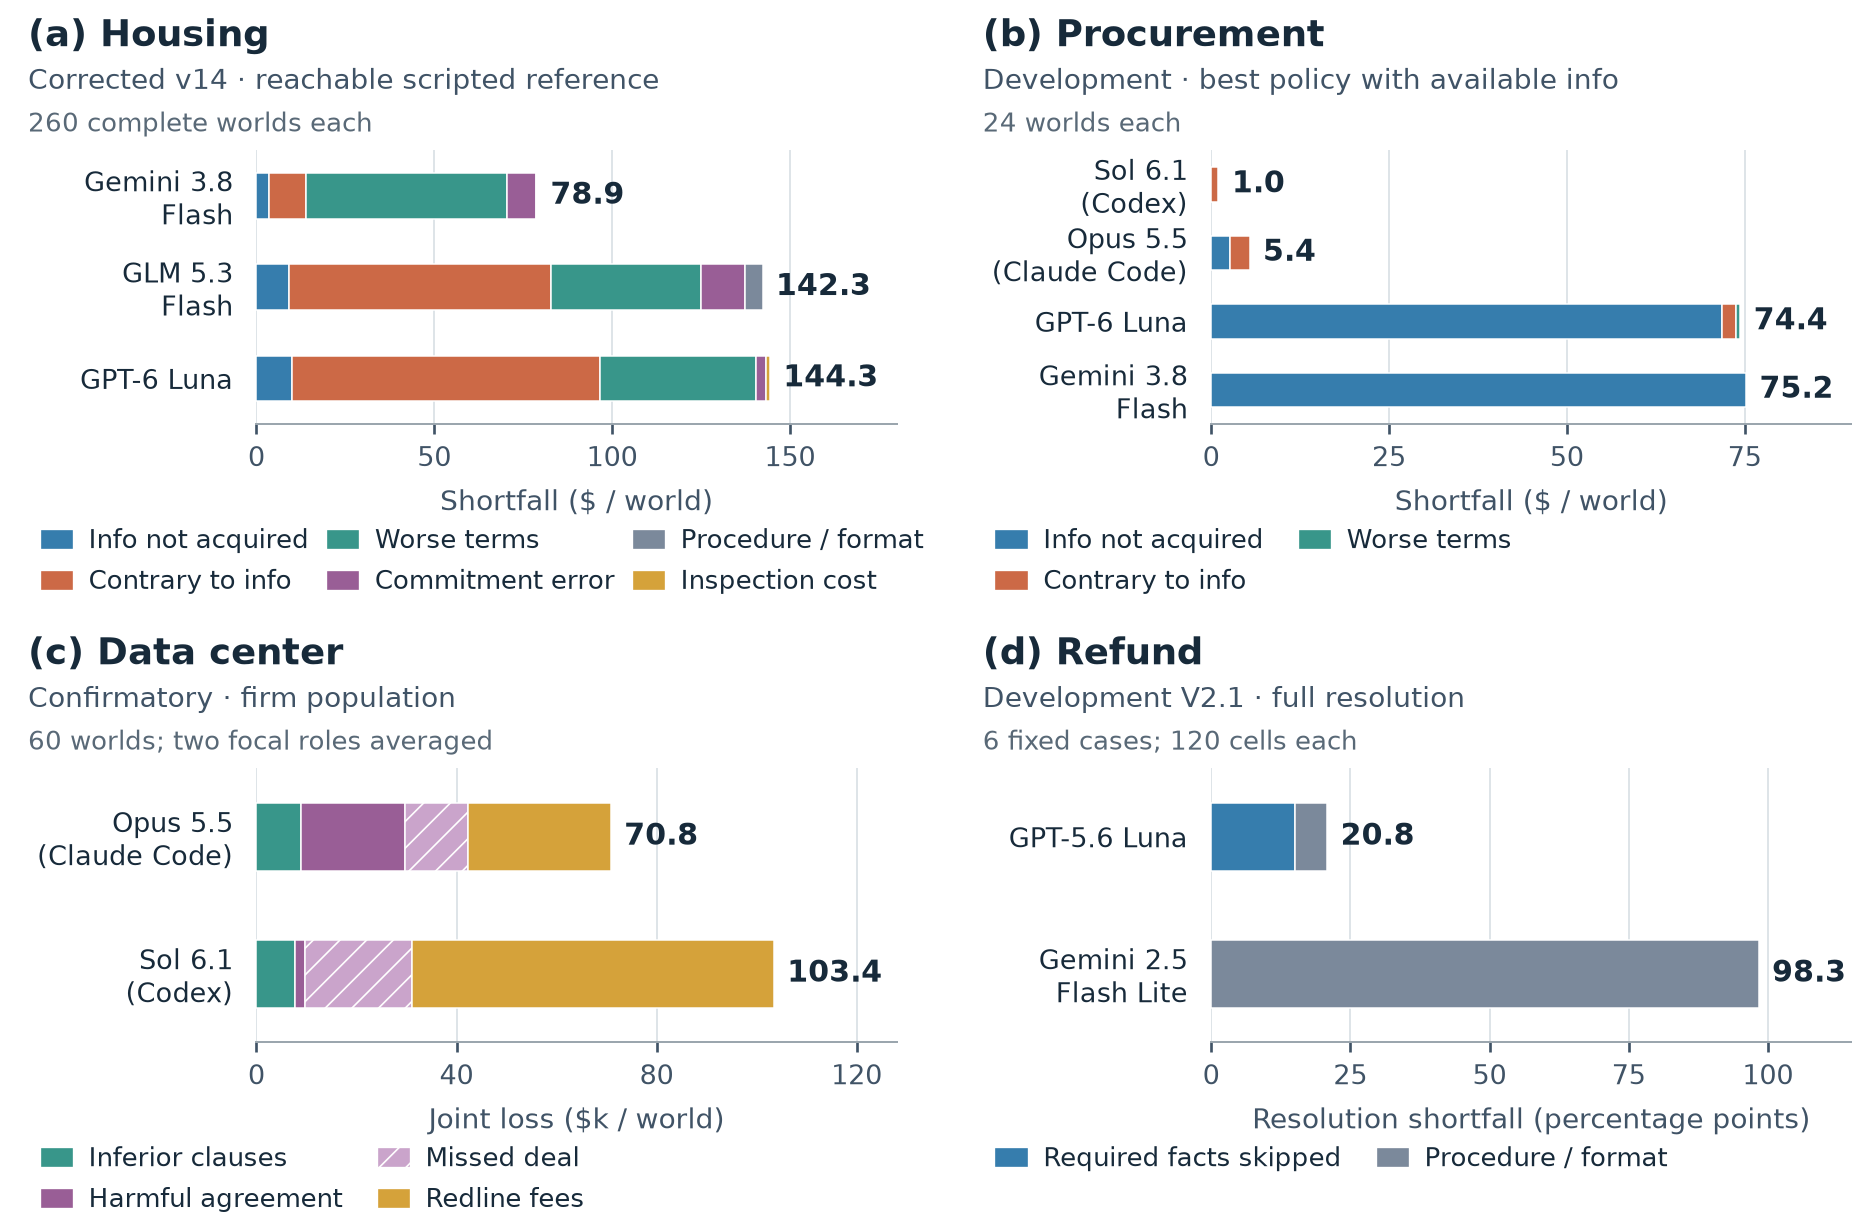
\includegraphics[width=\linewidth]{figures/shortfall_by_case.png}
\caption{\textbf{Shortfall to each case's reference.} Segments account for observed actions, and labels give mean totals
(lower is better within a panel). Units and scales differ across panels. Housing shows v15's two pre-registered models
and the three addendum subjects (A: GLM; B: Sol and Opus through their command-line tools) on the 260 main worlds of
Table 5.2, measured below the reachable scripted rule (\texttt{inspect\_\allowbreak{}lowball}, as in Table 5.2's fourth row); the few
negative amounts, at most \$0.4 a world, are in Table E.10 and are not drawn. Procurement shows all four subjects on
the 20 pre-registered worlds of Table 5.3; full subject tables are in Appendix E.5. Data center reports v2's joint loss
relative to the full-information bound with the firm counterparts at \$25k per paid redline, across all 80 worlds of
Table 5.4 with both seats averaged. In Procurement, \$6.33 a world of Luna's information-not-acquired segment is the
worse-quantity part of awards made before a worthwhile test; the pre-registered classification rules file such an
award's whole loss under that class (Table E.10). Intervals and exact values appear in Tables 5.3, E.9 and E.10.}
\label{fig:5.2}
\end{figure}

The labels name what happened. The mechanism behind each large segment is as follows.

\textbf{Procurement: three models never test, and Sol secures the recorded supplier first.} Opus, Gemini and Luna asked
no newcomer for anything in any of their 120 plays: they requested quotes and samples from the recorded supplier and
awarded it the order, so nearly all of their loss is information not acquired, and the rest is award checks, each of
which spends an action. Luna's further \$6.85 a world comes from ordering 50 units where 55 was best in 15 of its 40
plays; the pre-registered classes file most of it under information not acquired (Table E.10). Sol's loss divides by
world. Where it never tested a newcomer that the best policy would have tested, it lost \$17.5 a world. Where it did
test, it often first requested a quote and a sample from the recorded supplier, spending days and actions before the
newcomer test that the stated odds and clock made best (\$8.9 a world), or it awarded the order while a newcomer test
it had begun was still worth finishing (\$3.2).

\textbf{Housing, Gemini: it drops a known lemon even where the lemon is the better lease.} Worse terms account for 80\% of
its shortfall relative to the reachable rule (\$40.7 of \$51.1 a world), and nearly all of it comes from one move. Under
the landlord kind that prices a lemon from its own lower cost, a lemon's landlord counters about \$1,000 below a sound
listing's floor (\$995 to \$1,000 in these worlds), so a known lemon signed at that counter is worth what the listing
would be worth sound at a sound floor. This holds exactly in 187 of the 200 worlds whose favourite is a lemon, and
within \$5 in the rest. The rule inspects the favourite, finds the lemon, offers \$0 and signs the counter in all 200.
Gemini also inspected the favourite and found the lemon in all 200, but made an offer on it in only 4; in 172 episodes
it leased a sound listing that left it with less (\$65.0 a world). Under the other landlord kind the rule leases nothing
in 77 worlds, and Gemini's leases there offset \$26.5 a world. Gemini does read landlords' replies: of 74 replies that
proved a lemon, it walked away from 64 and signed above the lemon's value once. Ending with no lease where the rule
leased costs a further \$8.9 (12 of 520 episodes).

\textbf{Housing, Luna: it drops the lemons worth taking and signs ones that cost it.} Its shortfall relative to the
reachable rule is \$99.9 a world. Worse terms (54\%, \$54.3) follow Gemini's pattern: in the same 200 worlds Luna found
the lemon favourite in 197 and made an offer on it in 7, and in 154 episodes it leased a sound listing that left it
with less (\$57.7 a world). Signing a listing that a landlord's reply had proved a lemon accounts for 22\% (\$22.2,
11 episodes): the landlord accepted Luna's offer at a rent that no sound landlord would take, which by the stated
pricing rule proves a lemon, and Luna signed at that rent, above the lemon's value. Of 89 such replies, it walked away
from 58 and signed 20 at or below the lemon's value. Another 15\% (\$14.9, 64 episodes) comes from signing without
settling quality under the landlord kind whose replies reveal nothing, where an inspection was worth its \$25 fee every
time; 21 of those listings were lemons. Ending with no lease where the rule leased costs \$8.6. In v14, whose task
prompt did not state how landlords price, the reply-proved lemon accounted for 60\% of Luna's shortfall.

\textbf{Housing, Sol and Opus (addendum B): what remains is the price.} Neither lost anything by acting against what it
knew, and neither left a worthwhile inspection undone, apart from Opus's \$1.4 a world. Worse terms account for all of
Sol's \$15.3 shortfall (\$15.7, offset by \$0.4 of inspection fees it saved) and for 84\% of Opus's \$46.1 (\$38.8); ending
with no lease where the rule leased costs Opus a further \$6.3.

\textbf{Refund, Gemini 2.5 Flash Lite: the case ends before it decides.} In 81\% of its episodes it asked again for a fact
it had already been given; the environment rejects a repeated request, and the case ends with no decision (80.8 of its
98.3 points). In most of the remaining episodes it denied the claim correctly but wrote the refund method as null
where the policy's format requires ``none'' (16.7 points). It reached the answer key's outcome in 18\% of episodes and a
wrong outcome in none.

\textbf{Data center: fees, then deals the client walked away from.} Every redline after the opening move costs \$25k. The
full-information reference signs the best agreement at once, so each fee counts as loss, whichever side paid it.
Against the firm counterparts, across all 80 worlds with both seats averaged, fees account for 59\% of Sol's joint loss
(\$83.4k of \$140.2k a world) and 54\% of Opus's (\$45.3k of \$83.6k). Sol redlines more: as integrator it made 371
redlines to the firm client's 262, whereas Opus made 227 to 189. Some of those redlines buy better clauses, and a seat
that does not know the other side's costs may need them, so their share alone does not show wasted negotiation. Nearly
all of the remaining loss is deals lost in worlds that had one (35\% of Sol's loss and 34\% of Opus's), and every one of
them ended with the client walking away. With each model as integrator, the firm client walked away from Sol in 40 of
its 144 plays of deal worlds and from Opus in 14. As client, each model walked away in 26 of the 72 deal worlds. No
agreement was harmful: with the walk-away point in the task prompt, neither model signed in any of the 8 worlds
without a deal.

The pre-registered plan included a replay of the recorded moves at other fees, which shows what the same moves would
earn, not how the models would play. Without fees, Sol still loses more joint value than Opus against the firm
counterparts (\$63.1k against \$42.5k a world, seats averaged) and earns more in both seats. At \$50k a redline its
earnings fall below Opus's (as integrator 67.9 against 69.7, as client 1.3 against 22.8, in thousands of dollars per
deal world), because it redlines more. Appendix E.9 gives v1's fuller replay.

\textbf{Across the cases.} Four findings hold across the cases. First, the gap lies in a stratum that the design fixes in
advance, so every case reports by stratum and pools last. Second, the counterpart is part of the measurement, so a
claim names the counterparts it covers. Third, what the task prompt states moves the score as much as the subject does
(stating two rules cut procurement loss by \$11 to \$14; stating a walk-away cost cut losing signatures from 15 of 60 to
1 of 60), so the task prompt is a versioned part of the case. Fourth, a pattern found by looking back is a hypothesis
until a pre-registered test confirms it.

Housing, Procurement and Data center take their decision structure from real settings (Section 5.1): informal
rentals, wholesale sourcing and AI-infrastructure contracting. We set their parameters ourselves; they are not
calibrated to field data. The experiments use controlled scenarios and a small set of agent configurations, with no
human policy baseline, and they do not establish general model rankings.

\subsection{An external benchmark on the same runtime}\label{an-external-benchmark-on-the-same-runtime}

TERMS-Bench evaluates bilateral price negotiation against counterparts whose type is hidden \citep{zhang2026termsbench}. We reimplemented,
from the paper's description, its alternating-offer environment, three of its six counterpart families (Candid,
Taciturn and Expressive) and four of its measures as one AERead family. The counterpart runs as a scripted seat, and
its random draws are sealed each turn, so replay recomputes the counterpart's moves as well as the scores. We did not
implement the Oracle-Cue reference or the gap measures built on it, the urgency regime, type-belief error or the other
three families, and counterpart messages are templates. The corpus has 30 cases, 15 with a zone of agreement and 15
without, each played once.

\renewcommand{\thetable}{5.5}
\begin{longtable}[]{@{}
  >{\raggedright\arraybackslash}p{(\linewidth - 8\tabcolsep) * \real{0.1579}}
  >{\raggedleft\arraybackslash}p{(\linewidth - 8\tabcolsep) * \real{0.2105}}
  >{\raggedleft\arraybackslash}p{(\linewidth - 8\tabcolsep) * \real{0.2105}}
  >{\raggedleft\arraybackslash}p{(\linewidth - 8\tabcolsep) * \real{0.2105}}
  >{\raggedleft\arraybackslash}p{(\linewidth - 8\tabcolsep) * \real{0.2105}}@{}}
\caption{\textbf{TERMS-Bench reimplementation: two of the paper's agents on the same 30 cases, scripted
counterpart and settings. Agreement and surplus are computed over the cases with a zone of agreement: 15 for
GPT-4o-mini and 12 for GLM-5.1, whose three malformed moves removed those episodes. Paper values:
surplus efficiency from its Table 16 (overlap regime, mean of the three families played here);
agreement and conditional surplus efficiency from its Table 2, which pools six families and three
regimes.}}\label{tab:5.5}\tabularnewline
\toprule\noalign{}
\begin{minipage}[b]{\linewidth}\raggedright
\end{minipage} & \begin{minipage}[b]{\linewidth}\raggedleft
GPT-4o-mini
\end{minipage} & \begin{minipage}[b]{\linewidth}\raggedleft
GLM-5.1
\end{minipage} & \begin{minipage}[b]{\linewidth}\raggedleft
Paper: GPT-4o-mini
\end{minipage} & \begin{minipage}[b]{\linewidth}\raggedleft
Paper: GLM-5.1
\end{minipage} \\
\midrule\noalign{}
\endhead
\bottomrule\noalign{}
\endlastfoot
Agreement rate where a deal exists (AGR+) & 0.80 & 1.00 & 0.522 & 0.951 \\
Surplus efficiency (SE+) & 0.035 & 0.458 & 0.196 & 0.668 \\
Conditional surplus efficiency (CSE+) & 0.044 & 0.458 & 0.363 & 0.721 \\
\end{longtable}

The reimplementation orders the two agents as the paper does on all three measures, but absolute levels are lower for
both, and for a third model. A review of the port after these runs traced the shift to four departures from the
paper's protocol rather than to the agent, whose interface in the paper is also one stateless call per round. First,
our prompt does not state the agent's payoff or the rule against accepting above its reservation value. Second, its
observation differs from the paper's. Third, a malformed move removes the episode where the paper applies a fallback;
under that fallback, GLM-5.1's surplus efficiency would be 0.520 over all 15 cases. Fourth, our price range and zone
widths are wider than the paper's. We have built a pre-registered reproduction with those fixes, and it stopped at its
first check: one of the paper's fixed-concession baselines (FC10) scores 0.307 here against the paper's 0.266, while
the other two match. The paper states how much the baselines concede (1\%, 10\% or 30\% of the remaining distance per
offer) but not how they open or accept. No agent has played the reproduction. The paper reports critical violations
by GLM-5.1 in 5\% of cases without a zone of agreement for these three families; at that rate, 15 such cases would show
none about half the time, and ours showed none. The port also exposed a harness effect. On one provider route, any
specified reasoning budget suppressed deliberation, and GLM 5.3 Flash breached its own reservation value in 13 of
30 cases, against the paper's band of 0 to 2.06\%. With no reasoning setting specified, it breached in 2 of 30 and its
surplus efficiency rose from 0.40 to 0.53; the comparison above uses that setting. This is why the reasoning condition
is part of each run's frozen configuration. The runtime's support for the scripted seat that this family uses is now
on the main branch.
